\documentclass[final,pdftex]{../../template/epsilonj}

\RequirePackage{graphicx}
%\usepackage{microtype}

\RequirePackage[colorlinks,citecolor=blue,urlcolor=blue]{hyperref}

\startlocaldefs
\numberwithin{equation}{section}
\endlocaldefs

\addbibresource{epsilon1.bib}


\begin{document}
	
	% \microtypesetup{protrusion=false, expansion=false}
	\begin{frontmatter}
		\title{\protect{$p$}-value: то, что вы всегда хотели узнать, но боялись спросить}
		\runtitle{\textit{p}-value: то, что вы всегда хотели узнать}
		
		\begin{aug}
			\author{\imya{Мария} \fam{Лысюк}}
			\runauthor{М. Лысюк}
			\address{НИУ ВШЭ, Москва.}
		\end{aug}
		
		\begin{abstract}
			Аннотация должна передавать краткое содержание работы.
			Она должна быть ясной, содержательной, релевантной и~короткой
			(не более 150~слов). Аннотация должна содержать информацию,
			необходимую для поиска по базам научных работ. 
			В~аннотации не должно быть математических формул.
			
			Этот файл является образцом. Сравните его исходный код
			с~финальным PDF-файлом, чтобы получить представление о~том,
			как написать статью по данному шаблону.
		\end{abstract}
		
		\begin{keyword}
			\kwd{p-value}
			\kwd{уровень значимости}
			\kwd{гипотезы}
			\kwd{интерпретация}
		\end{keyword}
		
	\end{frontmatter}
	
	% \microtypesetup{protrusion=true, expansion=true}


С завидным постоянством хотя бы раз в жизни студент, слушающий курс статистики, сталкивается с вопросом экзаменатора (который обычно ещё надеется, что вопрос очевиден и «вытягивает» с помощью него студента): «Мистер $X$, что показывает $p$-value?»

И тут для многих наступает этот неловкий момент, и лицо выглядит примерно вот так (Эдвард Мунк, видимо, тоже не знал):

\begin{figure}[htbp]
	\centering
	
\includegraphics[width=8cm]{munk.jpg}
	\caption{Лицо обычного человека, у которого спросили, что такое $p$-value}
\end{figure}

Для того, чтобы осознать сие, безусловно, великое понятие, мы должны, как Будда, пройти 7 ступеней познания. Как водится, примеры красноречивее всего доносят нужную информацию до мозга, так что поговорим сегодня про машинки:)

Вкратце \textbf{о ходе эксперимента}. Мы будем узнавать, есть ли какая-то зависимость между тем, зависит ли лихачество водителей от цвета их машины. И гипотеза $H_o$ будет выглядеть следующим образом:

$H_0$: Выдача штрафа не зависит от цвета машины.

$H_1$: Водители с красными машинами чаще получают штрафы за превышение скорости по сравнению с синими машинами.


Итак, в добрый путь!

\textbf{Ступень 1. Выберите уровень значимости.} Начнем со знакомого до боли:) Строго говоря, уровень значимости- это мера, которая отражает наше желание относительно точности результатов- низкие уровни значимости говорят о маленькой вероятности того, что полученные экспериментальным путем результаты- случайны, и наоборот. Согласно конвенции, как правило, используется 5\% уровень значимости. Это означает, что вероятность того, что наши результаты случайны- 0.05, и 0.95, что мы сами повлияли на результат.

\begin{itemize}
	\item Пример: Возьмем и мы уровень значимости в 5\% :)
\end{itemize}

\textbf{Ступень 2. Определите ожидаемые результаты эксперимента.} Как правило, ученые, проводя эксперимент и наблюдая впоследствии результаты, имеют представление о том, какие результаты являются <<типичными>> до начала эксперимента. Это может быть основано на результатах прошлых исследований, достоверных источников, научной литературы, и т.д. Для вашего эксперимента определите ваши ожидаемые результаты любым из способов.

\begin{itemize}
	\item Пример: Пусть предыдущие исследования показали, что штрафы за превышение скорости чаще получают водители красных машин по сравнению с синими. Также пусть результаты по всей стране показывают превышение красными в отношении 2:1 в сравнении с синими. Мы же хотим узнать, применимы ли результаты, характерные ко всей стране, к нашему городу. Если мы возьмем рандомную выборку из 150 машинок, которым выписали штрафы, мы будем ожидать, что 100 машин будут красными, а 50 синими,\em{ если наша полиция выписывает штрафы согласно национальной тенденции}.
	
\end{itemize}

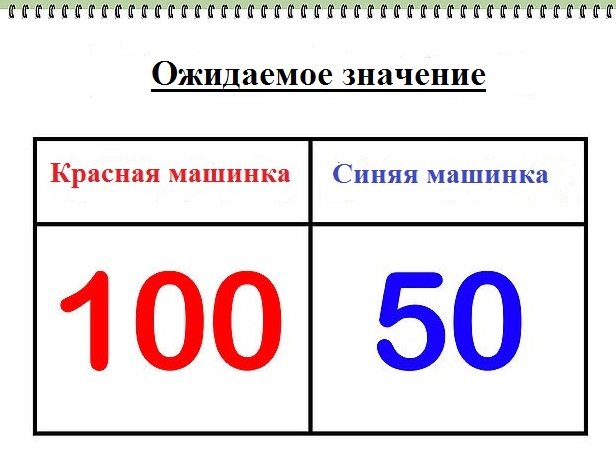
\includegraphics[width=100mm,height=70mm]{1.jpg}

\textbf{Ступень 3. Определите наблюдаемые результаты эксперимента.} После того как мы определили ожидаемые результаты, проводим реальный эксперимент и получаем наблюдаемые результаты. Если мы каким-либо образом повлияли и наблюдаемые результаты \em{отличаются} от ожидаемых, возможны 2 ситуации:

1) это произошло случайно

2) или те условия, в которых мы проводили эксперимент,\em{повлияли} на исход.

Как правило, цель нахождения p-значения- определить, правда ли что наблюдаемые результаты отличаются от ожидаемых настолько, что мы не можем отвергнуть нулевую гипотезу (гипотезу о том, что нет связи между переменными и наблюдаемым результатом).

\begin{itemize}
	\item Пример: Пусть уже в нашем городе мы произвольно выбрали 150 красных и синих машин-нарушителей. Оказалось, что 90 штрафов выписали красным машинам и 60 голубым. Это отличается от ожидаемых 100 и 50 соответственно. Правда ли, что те условия, в которых мы проводили эксперимент (в нашем случае смена источника данных с национальных на местные) послужила причиной изменения результатов, или действия городской полиции также смещены, как предсказывает национальная средняя оценка, и мы просто наблюдаем случайную вариацию? P-значение спешит на помощь!
\end{itemize}

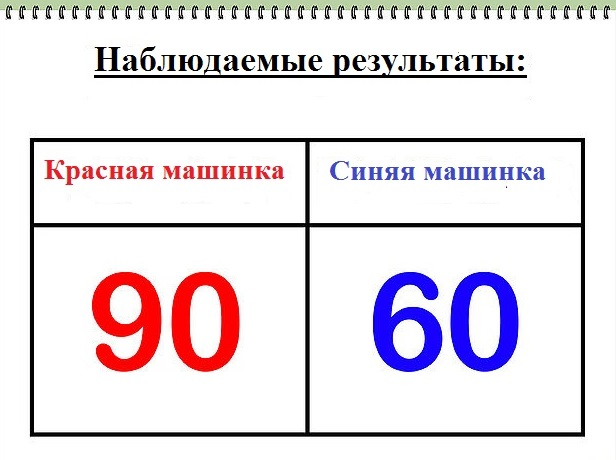
\includegraphics[width=100mm,height=70mm]{2.jpg}

\textbf{Ступень 4. Определите степени свободы в вашем эксперименте.} Степени свободы отражают меру изменчивости, характерную для исследования, которая определяется количеством переменных, которые вы изучаете. Степени свободы определяются как $n-1$, где n- это количество переменных, используемых в эксперименте.

\begin{itemize}
	\item Пример: У нас есть две переменных: красные машины и синие машины. Поэтому количество степеней свободы равно $2-1=1$.
\end{itemize}

\textbf{Ступень 5. Сравните наблюдаемые результаты с ожидаемыми с помощью $\chi^2$.} $\chi^2$- число, измеряющее разницу между ожидаемыми и наблюдаемыми результатами. Уравнение: 

$$\chi^2=\sum_{i=0}^{n} \cfrac {(h_i-e_i)^2}{e_i},$$

где h-значение наблюдаемой переменной, а е- ожидаемой.

\begin{itemize}
	\item Пример: Мы должны просуммировать значения для всех возможных переменных, то есть в нашем случае для синих и красных машинок.
\end{itemize}

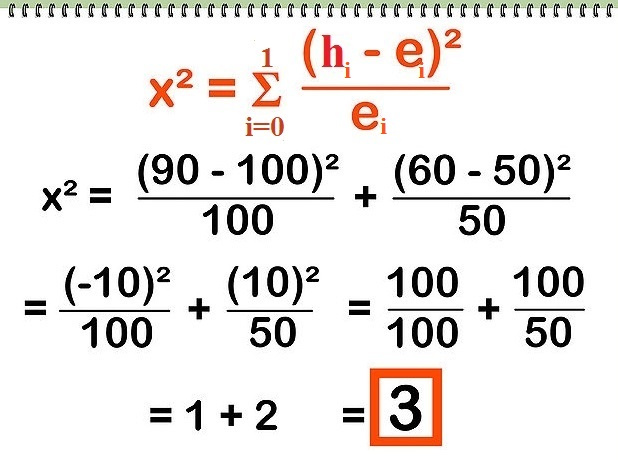
\includegraphics[width=100mm,height=70mm]{4.jpg}


\textbf{Ступень 6. Используем таблицу $\chi^2$- распределения, чтобы аппроксимировать значение p-value .} Скрестила пальцы: надеюсь, что все умеют пользоваться таблицами распределений:)

\begin{itemize}
	\item Пример: Наше значение $\chi^2=3$. Далее пользуемся таблицей для нахождения значения p-значение. У нас одна степень свободы, берем эту строку, и ищем там первое значение, превышающее значение нашего $\chi^2=3$. Итак, первое это 3,84. Соответствующее значение p-значения равно 0,05. Это означает, что наше p-value располагается в границах между 0.05 и 0.1.
\end{itemize}

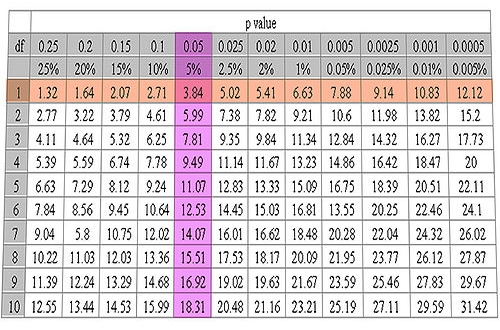
\includegraphics[width=150mm,height=90mm]{6.jpg}

\textbf{Ступень 7. Вот мы и добрались до конца! Осталось решить, отвергается или нет нулевая гипотеза.} Если значение p-значения меньше, чем уровень значимости, то мои поздравления (можете отсылать вашу работу в топовые журналы!), вы доказали, что вероятность того, что есть высокая корреляция между переменными, которыми вы манипулируете, и наблюдаемыми результатами, высока. Если ли же значение p-значение больше выбранного уровня значимости, вы не можете с точностью сказать,что полученные вами результаты случайны или являются результатом ваших действий.

\begin{itemize}
	\item Пример: Наше значение p-значение находится в границах от 0.05 до 0.1. Это означает, что это определенно меньше, чем выбранный уровень значимости, равный 0,05, поэтому, к сожалению, мы не можем отвергнуть нулевую гипотезу. Другими словами, мы не достигли желаемого уровня в 95\%, чтобы мы могли с точностью сказать, что в нашем городе полиция выдает штрафы красным и синим машинам в пропорции, значительно отличающейся от национального уровня. Иначе говоря, есть 5-10 \% вероятность того, что изменения в выдаче штрафов красным и синим машинам связано не со сменой локации, а по чистой случайности. В виду того, что мы ищем вероятность, меньшую чем 0.05, то мы не можем быть \em{уверны}, что полиция нашего города более склонна выдавать штрафы красным машинам, есть маленькая, но статистически значимая вероятность того, что это не так.
\end{itemize}

А теперь, после того как мы проделали такой дооооооооолгий путь к нирване, введем, наконец, определение:

P-значение- это вероятность того, что случайная величина с данным распределением (распределением тестовой статистики при нулевой гипотезе) примет значение, не меньшее, чем фактическое значение тестовой статистики.

И напоследок. Господин Goldman \footnote {Goodman S (2008). A Dirty Dozen: twelve p-value misconceptions. Semin Hematol 45(3):135–140} написал чудную статью о недопонимании относительно p-value и тех ошибках в интерпретации, которые обычно допускают студенты. \textbf{Не делайте так! Опасно для жизни!}

\begin{itemize}
	\item p=0.05 не означает, что есть 5\% вероятность того, что нулевая гипотеза верна
	\item p=0.05 не означает, что есть 5\% вероятность ошибки первого рода
	\item p=0.05 не означает, что есть 95\% вероятность того,что результаты будут такими же при повторении эксперимента
	\item p > 0.05 не означает, что нет разницы между наблюдаемыми переменными
	\item p < 0.05 не означает, что нулевая гипотеза не отвергается.
\end{itemize}

Источники:

http://www.wikihow.com/Calculate-P-Value

http://labstats.net/articles/pvalue.html	
	
\end{document}

